\documentclass[11pt, oneside]{article} 
\usepackage{geometry}
\geometry{letterpaper} 
\usepackage{graphicx}
	
\usepackage{amssymb}
\usepackage{amsmath}
\usepackage{parskip}
\usepackage{color}
\usepackage{hyperref}

\graphicspath{{/Users/telliott/Github/calculus_book/png/}}
% \begin{center} 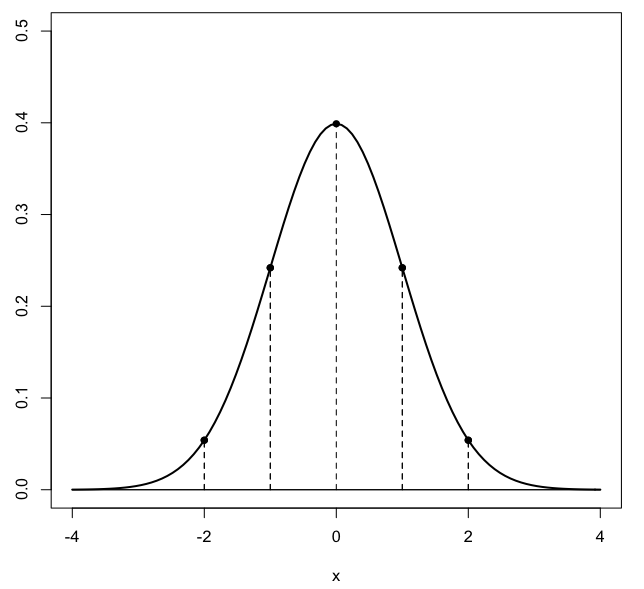
\includegraphics [scale=0.4] {gauss3.png} \end{center}

\title{Natural Numbers}
\date{}

\begin{document}
\maketitle
\Large
\section*{Integers}

The \emph{natural} or counting numbers which everyone learns very early in life are $1, 2, 3$ and so on.

One can get hung up on the question of whether the natural numbers would exist without the problem of counting three sheep or all ten of our fingers.  Leopold Kronecker said "God made the integers; all else is the work of man".

We will not worry about they come from.

Mathematicians refer to the \emph{set} of natural numbers and give this set a special symbol, $\mathbb{N}$.  We write
\[ \mathbb{N} = \{ 1, 2, 3 \dots \} \]

The brackets contain between them the \emph{elements} of the set.  The symbol $\in$ means "in the set" or "is a member of the set".

The dots mean that this sequence of numbers continue forever.

It seems hard to know how we can decide whether a particular $n$ is in the set if we can't enumerate all the members of the set.  But we can decide by its form whether $n$ is a natural number or not.  If this seems problematic, you might call $\mathbb{N}$ a \emph{class} instead (Hamming);  we carry out classification to decide whether $n$ is a natural number.

The notion of an unending sequence can be unnerving.  

\subsection*{construction of N}

To construct the set $\mathbb{N}$, start with the smallest element, $1$.  Then add successive elements by forming $a_{n+1} = a_n + 1$.

Sometimes people say that
\[ 0 \in \mathbb{N} \]
(0 is a part of the set), but most do not, and we will follow the definition given above.  If you wanted to be explicit about this you could write
\[ 0 \notin \mathbb{N} \]

$\mathbb{N}$ is an infinite set, meaning that there is no largest number in $\mathbb{N}$, no largest $n \in \mathbb{N}$.

Proof:  the proof is by contradiction.

We assume that the symbols and operations $>$ and $<$ are defined.

Suppose $\mathbb{N}$ does have a largest number, $a$.  Well, what about $a + 1$?  By the definition we can construct it, and it is clearly also a member of the set, but $a_{n+1} > a_n$ so $a_n$ is not the largest number in the set.

$\square$

What do we mean by infinity?  We mean a kind of bound on the numbers.  All numbers $n \in \mathbb{N}$ have the property that $n$ is contained in the interval $[1..\infty)$.  The right parenthesis means $\infty$ is \emph{not} part of the interval.  $\infty$ is \emph{not a number}!

\subsection*{least element}

A second important property of $\mathbb{N}$, as mentioned, is that there is a least number in the set.  If pairwise comparisons are carried out, a single element, the number $1$, has the property that $1 \le n$ for all numbers $n \in \mathbb{N}$.

\subsection*{well-ordered property}

Since we can also find the least member of the set excluding $1$, written $\mathbb{N} \setminus 1$, we can order every number in $\mathbb{N}$.  

This property is called the \textbf{well-ordered} property.

\subsection*{infinity is not a number}

One way of approaching this is to say, what goes wrong when we attempt to divide by zero?
\[ \frac{a}{0} = \ ? \]

Suppose 
\[ \frac{a}{0} = c \]
\[ a = 0 \cdot c \]

Equivalently, what number when multiplied by $0$ would result in $a$?

If there were such a number (say $\infty$), then what about 
\[ \frac{b}{0} = \ ? \]
\[ \frac{c}{0} = \ ? \]

By definition $0 \cdot a = 0$.  By definition, we do not allow division by zero.  And, by definition, \emph{infinity is not a number}.

\subsection*{limits}
Some people say that calculus is all about limits.  We will keep the discussion of limits and $\epsilon$-$\delta$ formalism to a minimum.  But let us try to establish an intuitive idea about what we mean when we say "in the limit as $N \rightarrow \infty$".

Above we had that there is no greatest integer.

A corollary of that is that in the limit
\[ \lim_{n \rightarrow \infty} \frac{(n + 1) - n}{n} = \ ? \]
As $n$ increases without bound, the difference between successive numbers, as a fraction of $n$, tends to zero.

To get an idea about this, first simplify by multiplying by $1/n$ on top and bottom.  Then
\[ \lim_{n \rightarrow \infty} \frac{(1 + 1/n - 1)}{1} = \frac{1}{n} = 0 \]

We say that $1/n$ \emph{tends} to zero as $n$ approaches $\infty$, and so does $[(n+1)-n]/n$.

\subsection*{the Integers}

The set $\mathbb{Z}$ contains all the members of $\mathbb{N}$ plus their negatives, as well as the special number $0$, often called the additive identity.

\[ \mathbb{Z} = \{ \dots -2, -1, 0, 1, 2, \dots \} \]

$\mathbb{Z}$ stands for the German word \emph{Zahlen}, Number.  The set $\mathbb{Z}$ are usually referred to as the integers.

$\mathbb{Z}$ is also an infinite set and also has the well-ordered property.  To show this simply order all numbers $p > 0$ with respect to zero using $<$, and all the numbers $n < 0$ using $>$.

\subsection*{inequality}
In the section above we used the symbols $>$ and $<$, greater than and less than, without introducing them.  I'm sure you've seen and used them before.  Among the axioms of the number systems is the collection of \emph{order axioms}.  As an example:

$\circ$ \ $x < y$ means that $y - x$ is positive

$\circ$ \ $y > x$ means that $x < y$

For arbitrary numbers $a$ and $b$ one of three statements is true:  

$a < b$, $a = b$ or $a > b$.

There is no intent to be systematic here.  Let us just mention that these properties (and their kin) are true not just for natural numbers, but also for the rational numbers and the real numbers, which we will talk about soon.  Here are just a few more important theorems in this class:

$\circ$ \ If $a < b$, and $c$ is any number, then $a + c < b + c$

$\circ$ \ If $a < b$, then $-b < -a$

$\circ$ \ If $a < b$ and $c > 0$, then $ac < bc$

\end{document}